\documentclass[a4paper,fleqn]{cas-dc}

% Numeric citation scheme ([1], [2], ...) to match \cite{} used below.
\usepackage[numbers]{natbib}
\usepackage{hyperref}
\usepackage{booktabs}
\usepackage{graphicx}
\usepackage{amssymb}
\usepackage{algorithm}
\usepackage{algpseudocode}
\usepackage{tikz}
\usetikzlibrary{arrows.meta,positioning,fit,backgrounds}

% \figslot{file.png}{width}{placeholder height}: includes the image when the
% file exists, otherwise draws a labelled box of the same size so the report
% still compiles and the layout stays honest before the figure is made.
\newcommand{\figslot}[3]{%
  \IfFileExists{#1}%
    {\includegraphics[width=#2]{#1}}%
    {\fbox{\parbox[c][#3][c]{\dimexpr#2-2\fboxsep-2\fboxrule\relax}{\centering\small Figure pending:\\ \texttt{\detokenize{#1}}}}}%
}

% =====================================================================
% Patch: cas-common.sty always prints "<authors>: Preprint submitted to
% Elsevier" in the running footer and an "ORCID(s):" footnote even when
% no \author has orcid= set. Both are overridden here rather than editing
% the class files, so the fix survives if those files are replaced.
% =====================================================================
\ExplSyntaxOn
\cs_gset:Npn \__first_footerline:
{
  \group_begin:
  \small
  \sffamily
  \ifnum\theblind>0\relax
  \else
    \__short_authors: :~
  \fi
  { \rmfamily \itshape NED~University~--~Information~Security~CEP }
  \group_end:
}
\ExplSyntaxOff
\RenewDocumentCommand \printorcid { } { }

\begin{document}
\let\WriteBookmarks\relax
\def\floatpagepagefraction{1}
\def\textpagefraction{.001}

\shorttitle{StreamShield: HTTP/2 stream-reset DoS detection and mitigation}
\shortauthors{S. M. Rayyan et al.}

\title[mode=title]{StreamShield: Detection and Mitigation of Indirection-based (HTTP/2 Stream-Reset) DDoS in Containerized Environments}

\author[1]{Syed Muhammad Rayyan (SE-23067)}
\author[1]{Maaz Ali Murtaza (SE-23092)}
\author[1]{Syed Ahmer Ali (SE-23099)}
\author[1]{Ali Afzal (SE-23048)}

\affiliation[1]{organization={Department of Software Engineering, NED University of Engineering and Technology},
                addressline={University Road},
                city={Karachi}}

\begin{abstract}
HTTP/2 stream-reset attacks turn the protocol's own multiplexing against the server: a single connection can open and tear down requests fast enough to exhaust a backend while sending very little over the wire. We build StreamShield, a self-contained, containerized system that reproduces, detects and mitigates two attacks in this class against a pinned, deliberately vulnerable Apache Tomcat 10.1.43. The first is Rapid Reset (CVE-2023-44487), where the client floods HEADERS followed by RST\_STREAM. The second is MadeYouReset (CVE-2025-8671), an indirection attack in which the client never sends a reset at all; it sends specification-legal but invalid control frames that make the server reset its own streams while the backend keeps processing the already-dispatched request. One detector watches two signals. An EWMA-smoothed client reset rate catches Rapid Reset, and a backend mismatch ratio, defined as in-flight requests over open protocol streams, catches MadeYouReset. In a three-scenario evaluation on the same victim, a legitimate traffic burst trips neither signal, Rapid Reset drives the reset rate from 0 to roughly 600 resets per second, and MadeYouReset drives the mismatch ratio from near 1 to over 100 while the client reset rate stays at exactly 0, which is the detection gap made visible. Mitigation is a layer-4 guard that blocks the offending source on alert; after enforcement both signals drain back to baseline and the victim keeps serving honest clients, which a separate legitimate-user probe quantifies as a recovered success rate and latency. Beyond blocking by source, StreamShield also implements a connection-scoped defence that serves an ENHANCE\_YOUR\_CALM GOAWAY to any single connection exceeding a reset budget, the per-connection approach the Rapid Reset disclosures recommend, which needs no source attribution and so applies equally to the indirection attack. The system is reproducible with Docker Compose and refuses any target outside the lab network.
\end{abstract}

\begin{keywords}
HTTP/2 \sep denial of service \sep Rapid Reset \sep MadeYouReset \sep Phantom Streams \sep stream reset \sep containerized testbed \sep intrusion detection \sep availability \sep Docker \sep Apache Tomcat
\end{keywords}

\maketitle

% =====================================================================
% 1. INTRODUCTION
% =====================================================================
\section{Introduction}\label{sec:introduction}

Availability is the part of the security triad that an attacker can break without ever reading or changing a single byte of protected data. A server that is too busy answering junk to answer its real users has already failed, and denial-of-service (DoS) techniques that reach this state cheaply are the ones worth studying. HTTP/2 made many of these techniques cheaper. Its multiplexing lets a client carry many concurrent requests, called streams, over one TCP connection, and it lets either side cancel a stream at any time with a RST\_STREAM frame \cite{rfc9113}. That cancellation is a normal, useful feature. It is also the lever behind a family of attacks in which the work of setting up and processing a request is paid for by the server while the work of cancelling it is nearly free for the attacker.

The best known member of this family is HTTP/2 Rapid Reset, disclosed as CVE-2023-44487 in October 2023 by Google, Amazon and Cloudflare after it was used to drive the largest DoS attacks recorded at the time, peaking in the hundreds of millions of requests per second \cite{rapidresetCloudflare,cisaRapidReset}. The pattern is simple: open a stream with a HEADERS frame, then immediately cancel it with RST\_STREAM, and repeat. Each cancelled stream frees its slot against the connection's concurrency limit at once, so the attacker never hits the ceiling the limit is supposed to enforce, and the server keeps allocating request-handling work for requests that are torn down a moment later.

A later and subtler member of the family motivates the term this project is framed around. MadeYouReset, disclosed as CVE-2025-8671 in August 2025 and tracked for Apache Tomcat as CVE-2025-48989, is an indirection attack \cite{madeyouresetCloudflare,certccMadeYouReset,cve20258671,cve202548989}. The attacker does not send a single RST\_STREAM. Instead it sends the server a control frame that is legal to send but invalid in context, for example a flow-control window update of zero, and the server responds to that protocol violation by resetting the stream itself. The reset is real and the protocol slot is freed, but the request on that stream was already dispatched to the application, so the backend goes on doing the work. The attack's authors name this protocol-closed-but-still-running stream a Phantom Stream, and identify the divergence between protocol-layer stream state and backend execution as the shared root cause of both attacks \cite{madeyouresetPaper}. The attacker has induced the damage indirectly, through the server's own correct error handling, which is exactly the shape the rubric names indirection-based DDoS (IDDoS). It also defeats any defence that watches for client-sent resets, because there are none to see.

Both attacks matter more, not less, in a containerized deployment. Containers share a host kernel and are given hard resource ceilings through control groups, so a backend thread pool or memory allowance saturated by phantom work is capped exactly where the operator set it, and a single busy container can starve its neighbours on the same host before any network-layer counter looks abnormal \cite{dockerDocs}. The same properties that make containers easy to pack densely make them easy to exhaust precisely, and the protocol-level nature of these attacks means a volumetric, request-per-second view can stay quiet while the service behind it falls over.

This report presents StreamShield, a complete system delivered as a Docker Compose stack, that treats both attacks end to end: reproduce, detect, then mitigate, with a quantitative before-and-after evaluation. The contributions are the following.

\begin{itemize}
  \item A containerized, reproducible testbed built around a pinned pre-patch Apache Tomcat 10.1.43 that is vulnerable to both attacks, with a lab-fenced traffic generator that produces legitimate load, Rapid Reset, and genuine MadeYouReset using crafted raw HTTP/2 frames.
  \item A single detector that carries two signals, an EWMA-smoothed client reset rate for Rapid Reset and a backend mismatch ratio for MadeYouReset, which together cover an attack that reset-rate monitoring alone cannot see.
  \item A mitigation point, a layer-4 guard in front of the victim, that blocks the offending source on alert and demonstrably restores service, driven either by one dashboard click or automatically.
  \item A three-scenario evaluation that derives the alert thresholds from measured data rather than assuming them, and that shows the detection gap directly by holding a legitimate load spike below both thresholds while each attack crosses the one that applies to it.
  \item An implementation, inside the same testbed, of the now-standard per-connection stream-reset-limit defence, which serves a forceful GOAWAY with the ENHANCE\_YOUR\_CALM code to any single connection whose reset count exceeds a budget. We do not claim this defence as new; vendors adopted it after MadeYouReset \cite{madeyouresetPaper}. We include it to compare source-level and connection-level enforcement directly, and to show that, acting on the connection rather than the source address, it needs no per-source attribution and so covers MadeYouReset as readily as Rapid Reset.
  \item A legitimate-user availability probe that measures the success rate and latency a real client experiences at the victim, so the effect of an attack and of mitigation is quantified as service availability directly, rather than only through the detector's internal signals.
  \item A direct phantom-stream count as a companion to the ratio, and a paced-attacker experiment that identifies a regime in which a slowed MadeYouReset stays under the reset-limit budget, so the standard fix never fires, while the divergence signal still detects it. A detection-quality harness reports detection latency and false-positive rate over repeated trials, and a calibration tool derives the thresholds from the measured benign baseline rather than assuming them.
\end{itemize}

The rest of the report is organised around these steps. Section~\ref{sec:background} explains the attack mechanisms, their effect in containerized environments, and the threat model. Section~\ref{sec:testbed} describes the testbed architecture and Section~\ref{sec:attacks} how each attack is reproduced and simulated. Section~\ref{sec:detection} covers the detection design, Section~\ref{sec:mitigation} the mitigation strategy, and Section~\ref{sec:evaluation} the quantitative evaluation. Section~\ref{sec:discussion} states the limitations honestly, and Section~\ref{sec:conclusion} concludes.

% =====================================================================
% 2. BACKGROUND AND THREAT MODEL
% =====================================================================
\section{Background and threat model}\label{sec:background}

\subsection{HTTP/2 streams and the reset primitive}\label{sec:http2-background}

HTTP/2 carries requests as independent streams multiplexed over one TCP connection \cite{rfc9113}. A client opens a stream by sending a HEADERS frame, the two endpoints exchange DATA frames, and the stream closes when both sides are done. Two features of this design are load-bearing for the attacks studied here. The first is the concurrency limit: a server advertises SETTINGS\_MAX\_CONCURRENT\_STREAMS to cap how many streams a client may have open at once, which is meant to bound the work the client can demand in parallel. The second is stream cancellation: either side can send a RST\_STREAM frame to abort a stream immediately, which is a legitimate feature for a client that, for example, navigates away from a page before its images finish loading.

The gap the attacks exploit is the mismatch between when a stream's protocol slot is released and when the work it created actually stops. A RST\_STREAM frees the slot against the concurrency limit at once, but if the request on that stream has already been handed to the application, the application does not necessarily stop. The attacker can therefore cycle through the concurrency limit far faster than the limit intends, because each slot is reclaimed the instant it is cancelled while the server-side cost it triggered is still being paid.

\subsection{Rapid Reset (CVE-2023-44487)}\label{sec:rapidreset-background}

Rapid Reset is the direct form of the attack. On each stream the attacker sends a HEADERS frame carrying a complete request, which causes the server to begin processing it, and then immediately a RST\_STREAM to cancel that stream. The loop repeats as fast as the connection allows. Because every cancellation frees a concurrency slot instantly, the attacker never settles at the advertised maximum and the server is pushed to allocate request-handling resources for a stream of requests that are each abandoned a moment after they start \cite{rapidresetCloudflareTech}. The asymmetry is the point: a HEADERS plus RST\_STREAM pair is a few dozen bytes for the attacker, while the server pays thread scheduling, request parsing and application dispatch for each one. In the 2023 disclosures this asymmetry produced record DoS volumes from comparatively modest botnets \cite{rapidresetCloudflare,cisaRapidReset}. The defining observable is that the resets come from the client, so a counter of client-originated RST\_STREAM frames rises sharply during the attack.

\subsection{MadeYouReset (CVE-2025-8671): the indirection case}\label{sec:madeyoureset-background}

MadeYouReset reaches the same exhausted state while removing the one observable that made Rapid Reset catchable. The attacker opens a stream and sends a complete request as before, so the backend dispatches it, but it never sends RST\_STREAM. Instead it sends a control frame that the specification allows on the wire but that is invalid in the current context, and the server, following its own correct error handling, resets the stream for the attacker, which never sends a reset of its own \cite{madeyouresetCloudflare,imperva}. Against the pinned Tomcat in this lab three such frames produce a clean per-stream reset: a WINDOW\_UPDATE with an increment of zero, a WINDOW\_UPDATE that overflows the flow-control window past its maximum, and a PRIORITY frame of the wrong length. Each is a protocol violation scoped to a single stream, so the server answers with a stream-level RST\_STREAM rather than tearing down the whole connection. Figure~\ref{fig:sequence} sets the two frame sequences side by side.

\begin{figure*}[t]
\centering
\figslot{figs/sequence.pdf}{\textwidth}{0.45\textwidth}
\caption{Frame sequences of the two attacks on one connection. Left: in Rapid Reset the client sends HEADERS and then its own RST\_STREAM on every stream. Right: in MadeYouReset the client sends HEADERS and a crafted WINDOW\_UPDATE with increment 0, and the server sends the RST\_STREAM. In both cases the backend work started by the request keeps running after the stream is reset.}
\label{fig:sequence}
\end{figure*}

The consequence is what the lab calls a phantom stream. The protocol layer considers the stream closed the moment the server resets it, and the slot against the concurrency limit is freed, yet the request on that stream was already dispatched and the application keeps running it to completion. The access log confirms this directly: a stream reset about a millisecond after it opens still records a full backend service time for its request before it is finally recycled. The attacker thus accumulates application-layer work that is invisible at the protocol layer, bypasses the concurrency limit exactly as in Rapid Reset, and, because it sends no resets of its own, leaves a client-reset counter sitting at zero throughout. This is why the attack is correctly called indirection-based: the harmful reset is performed by the server, induced by a frame that is not itself a reset. Figure~\ref{fig:phantom} shows the two lifetimes on one time axis.

\begin{figure}[t]
\centering
\figslot{figs/timeline.pdf}{\columnwidth}{0.5\columnwidth}
\caption{A phantom stream with the work endpoint set to 500\,ms. The HTTP/2 stream is reset about 1\,ms after it opens and its concurrency slot is freed, but the backend request keeps running for the full 500\,ms. That leftover work is what the mismatch ratio of Section~\ref{sec:signal-mismatch} counts.}
\label{fig:phantom}
\end{figure}

\subsection{Why containerized environments sharpen the impact}\label{sec:container-impact}

A container is a process tree under a hard resource ceiling imposed by control groups, typically a CPU share and a memory limit set by the operator \cite{dockerDocs}. That ceiling is the feature these attacks turn into a weapon. The phantom work of either attack consumes worker threads and memory inside the victim container, and because the container cannot grow past its cgroup limit, saturation happens precisely at the configured boundary rather than being absorbed by spare host capacity. On a shared host, one saturated container degrades the containers packed next to it, a noisy-neighbour failure that spreads from a single exploited service. In an autoscaling deployment the same pressure instead converts into cost, because the orchestrator reads the saturation as genuine demand and schedules more replicas to serve requests that are never completing. In each case a network-layer, requests-per-second view of the traffic can look ordinary while the service behind it is failing, which is the gap the detection in this report is built to close.

\subsection{Threat model and scope}\label{sec:threat-model}

The attacker is a remote client that can open HTTP/2 connections to the victim and send arbitrary, including malformed, frames on them. It does not have credentials on the victim, cannot run code on the host, and does not sit on the network path between other clients and the victim, so it cannot observe or modify their traffic. Its goal is denial of service: to exhaust the victim's request-handling capacity so that legitimate clients are refused or badly delayed. This matches both CVEs, which are unauthenticated, network-reachable availability vulnerabilities \cite{cve20258671,cve202344487}.

The defender controls the deployment: the victim container, a proxy in front of it, and a monitoring and enforcement path alongside. The defender does not get to patch the victim, which is the premise of the lab, since the point is to detect and mitigate the attacks at the deployment layer against a server that remains vulnerable. Detection may read the victim's own telemetry and the proxy's connection state; mitigation may act at the proxy. Out of scope are attacks that compromise the host or the container runtime, volumetric floods that saturate the network link before any of this logic applies, and application-logic abuse unrelated to the stream-reset mechanism. The whole lab runs on a private Docker bridge network, the victim is treated as radioactive and never exposed outside it, and the traffic generator refuses any target that does not resolve to a loopback or private address, with no override, so the techniques cannot be pointed at a system the operator does not own.

% =====================================================================
% 3. TESTBED ARCHITECTURE AND IMPLEMENTATION
% =====================================================================
\section{Testbed architecture and implementation}\label{sec:testbed}

\subsection{Design goals}\label{sec:testbed-goals}

The testbed has to satisfy four requirements at once. It must be reproducible, so a marker can bring the whole stack up with one command and get the same behaviour. It must be isolated, so a deliberately vulnerable server never touches a real network. It must stay vulnerable, because the exercise is to detect and mitigate the attacks at the deployment layer rather than to patch them away. And it must be observable at two layers, the HTTP/2 protocol layer and the application layer, because, as Section~\ref{sec:madeyoureset-background} showed, the MadeYouReset signal lives in the divergence between the two. The stack is a Docker Compose project that meets all four: one command builds and starts it, every service sits on a private bridge network, the victim is pinned to a pre-patch release, and two independent measurement paths read the protocol state and the real backend work.

\subsection{Services and data flow}\label{sec:services}

The lab is six containers on one internal bridge network named \texttt{h2lab-net}, plus an optional two-container metrics stack. Table~\ref{tab:services} lists each service and its job. Traffic enters at the guard, which proxies it to the victim; the victim writes protocol-level debug logs and serves an application-layer inflight counter; the exporter turns both into metrics; the detector scrapes the exporter and the guard once per second, decides whether an attack is in progress, and can drive the guard to block a source; and the dashboard shows the live state and offers a mitigation control. The attacker container is launched on demand rather than run continuously, which keeps the baseline clean.


\begin{table*}[t]
\centering
\caption{Services in the containerized testbed. All run on one private bridge network; only the dashboard and the guard entrypoint are published to the host.}
\label{tab:services}
\begin{tabular}{@{}lll@{}}
\toprule
Service & Role & Key detail \\
\midrule
victim & Deliberately vulnerable server & Pinned Apache Tomcat 10.1.43, h2c, backend-work endpoint \\
victim-exporter & Protocol and app-layer signals & Tails the HTTP/2 debug log, exposes Prometheus metrics \\
guard & Proxy and enforcement point & Layer-4 TCP proxy with a source blocklist \\
detector & Detection and decision & Scrapes every second, two signals, drives mitigation \\
dashboard & Operator view and control & Live charts, alert banner, mitigate control (loopback only) \\
attacker & Lab traffic generator & Legitimate load, Rapid Reset, MadeYouReset; lab-fenced \\
\midrule
prometheus, cadvisor & Optional history and host view & Time-series store and per-container CPU/memory \\
\bottomrule
\end{tabular}
\end{table*}

\subsection{The vulnerable victim}\label{sec:victim}

The victim is Apache Tomcat 10.1.43 running on a JDK 17 base image. The version is pinned on purpose: 10.1.43 is the last 10.1.x release before the MadeYouReset fix landed in 10.1.44, so it is vulnerable to both attacks and stays that way for the life of the lab \cite{cve202548989}. HTTP/2 is served over cleartext (h2c) on a single connector, which removes TLS certificate handling from the lab without changing the behaviour under study, because the stream-reset mechanics live at the frame layer and are identical whether or not the connection is encrypted. The connector advertises \texttt{maxConcurrentStreams} of 100, a modest cap so that the per-connection stream limit, the control both attacks are designed to slip past, is small enough to see in the metrics.

Two pieces of instrumentation make the victim observable. The application it serves is a single endpoint that simulates backend work: a request to \texttt{/?ms=N} occupies a worker thread for \texttt{N} milliseconds before replying, which stands in for real processing and sets how long a phantom stream keeps a thread busy after its protocol stream is gone. Alongside it, a small Tomcat valve maintains the real in-flight request count. The valve increments when a request enters the pipeline and decrements only when that call truly returns, after the servlet has finished, so it tracks whether a backend thread is still working regardless of what the HTTP/2 layer has decided about the stream. This matters because stock Tomcat 10.1.43 exposes no equivalent request-level in-flight count over JMX; the valve is what makes the application-layer half of the MadeYouReset signal measurable, and it is the divergence between this count and the protocol-layer stream count that the detector in Section~\ref{sec:detection} keys on.

\subsection{A configuration correction found during reproduction}\label{sec:overhead}

Reproducing MadeYouReset cleanly needed one correction that is worth recording, because it shows the attack interacting with a real defence. Tomcat ships an HTTP/2 overhead protection that counts cheap or abnormal frames and closes the whole connection once a connection crosses an overhead budget. With that protection active, the crafted frames of Section~\ref{sec:madeyoureset-background} did not produce the clean per-stream reset the attack depends on; instead Tomcat raised a connection-level error and sent GOAWAY, tearing down the connection before any phantom streams could accumulate. The lab's intent is to disable this protection so the stream-reset mechanism can be studied in isolation, and the connector is configured accordingly. The subtlety is that Tomcat disables the protection for any factor below 1, but a first attempt using a value of $-1$ did not take effect as expected, and the crafted frames kept tripping the connection-level close. Setting the overhead factors to 0 disables the protection as intended, after which the three usable primitives reset streams cleanly one at a time.

This is more than a configuration note. Tomcat's overhead protection reacting to the crafted frames is itself a coarse, connection-level defence against this class of attack: it will eventually drop a connection that is behaving abnormally. The lab disables it deliberately so that the finer, backend-side detection, which identifies the attack without killing the connection and without the false positives a blunt overhead counter would produce under legitimate bursty load, can be studied on its own. The coarse defence and the fine one are complementary, and the report returns to this in the discussion.

\subsection{Isolation and safety by construction}\label{sec:isolation}

The lab is built so the vulnerable server cannot escape it. Every container is attached only to the private bridge network, and the sole ports published to the host are the guard entrypoint, for local testing against the victim, and the dashboard. The dashboard is bound to loopback explicitly rather than to all interfaces, because it holds the Docker socket so its buttons can launch attack containers, which makes it root-equivalent host control that must never be reachable from the local network. The victim itself exposes nothing to the host at all. These measures keep a pinned, intentionally vulnerable Tomcat sealed inside the lab, where it is meant to stay.

% =====================================================================
% 4. ATTACK SIMULATION
% =====================================================================
\section{Attack simulation}\label{sec:attacks}

\subsection{The traffic generator and its lab fence}\label{sec:generator}

A single tool generates every workload the lab uses: an idle baseline, legitimate load, Rapid Reset, and MadeYouReset. Before any mode runs it checks the target, and it refuses to proceed unless the host is a lab service name or resolves to a loopback or private (RFC 1918) address. There is no flag to override this. The refusal is the software enforcing the scope of Section~\ref{sec:threat-model}: the techniques it implements are harmful against systems one does not own, so the tool will only ever point at the local victim. The four modes map directly onto the evaluation scenarios of Section~\ref{sec:evaluation}, which lets the same tool produce both the controls and the attacks under identical conditions.

\subsection{Legitimate load as the control}\label{sec:legit}

The legitimate mode opens several honest HTTP/2 connections and sends well-formed requests to the work endpoint, completing each one normally. It is the control that the detection has to get right: a genuine traffic burst looks busy, drives real backend work, and must not trip either alert. Running it against the same victim as the attacks is what lets the evaluation answer the obvious objection, that the detector simply fires on any load, with a measurement rather than an assertion.

\subsection{The Rapid Reset engine}\label{sec:rapidreset-engine}

Rapid Reset is produced with a standard HTTP/2 client library, because every frame it sends is well formed. Each worker holds one connection and loops: send a HEADERS frame carrying a complete GET, with the end-of-stream flag set so the server dispatches the request, then immediately send RST\_STREAM with the CANCEL code to abort that same stream. The loop advances the stream identifier and repeats as fast as the connection allows, recycling the connection before the identifier space runs out and draining the socket occasionally so it does not stall. The effect on the victim is the one described in Section~\ref{sec:rapidreset-background}: the server does per-request setup for a stream of requests that are each cancelled a moment later, while the concurrency slot is freed instantly on every cancellation. The defining observable is that the resets come from the client, which is what the reset-rate signal of Section~\ref{sec:detection} measures.

\subsection{The MadeYouReset engine}\label{sec:madeyoureset-engine}

MadeYouReset cannot be produced with a high-level client, because a conformant library will not emit the malformed frames the attack depends on. The tool therefore speaks HTTP/2 over a raw socket, using an HPACK encoder only to build the request header block, and constructs the crafted frames byte by byte. Each worker opens a stream, sends a complete GET so the backend dispatches the request, and then sends exactly one crafted frame that makes the server reset that stream. It never sends RST\_STREAM itself. Between streams it services the socket to acknowledge the server's settings and ping frames and to tally the server-sent resets it provokes, and it can pace itself with a configurable gap so the run is controlled and reproducible rather than an uncontrolled flood. Across the run the worker accumulates phantom streams: protocol slots freed by the server's resets while the corresponding backend threads keep running the dispatched requests to completion.

\subsection{Primitives and the probe}\label{sec:primitives}

The MadeYouReset literature lists five candidate frames that should provoke a server reset. Not all of them behave the same way against a given server, so the tool includes a probe mode that sends each candidate once and reports whether this Tomcat answers with a stream-level reset, which is a usable trigger, or a connection-level error, which is not. Table~\ref{tab:primitives} gives the result for the pinned victim. Three of the five produce clean per-stream resets and are usable; the other two, a HEADERS or DATA frame on a half-closed stream, are treated by this Tomcat as connection errors and close the whole connection, so they cannot accumulate phantom streams. The default primitive is the zero-increment window update. Reporting this honestly, rather than assuming all five land, is part of what makes the simulation faithful to the specific server under test.

\begin{table*}[t]
\centering
\caption{MadeYouReset primitives against the pinned Tomcat 10.1.43, as reported by the probe. A stream-level reset is a usable trigger; a connection-level error is not.}
\label{tab:primitives}
\begin{tabular}{@{}lll@{}}
\toprule
Primitive & Crafted frame & Result \\
\midrule
Zero-increment & WINDOW\_UPDATE increment 0 & stream reset (usable) \\
Window-overflow & WINDOW\_UPDATE past $2^{31}-1$ & stream reset (usable) \\
Priority-length & PRIORITY of wrong length & stream reset (usable) \\
Headers-half-closed & HEADERS on a half-closed stream & connection error \\
Data-half-closed & DATA on a half-closed stream & connection error \\
\bottomrule
\end{tabular}
\end{table*}

\subsection{Reproducing a run}\label{sec:reproduce}

Each workload is a single command through a helper script, so a run is reproducible end to end. After the stack is up, one invocation produces legitimate load, another runs the probe to confirm which primitives land on the current victim, and another runs a sustained Rapid Reset or MadeYouReset with a chosen connection count, duration and backend-work time. The parameters that shape an attack, how many connections, which primitive, how long each request occupies a thread, and the pacing gap, are all explicit arguments, which means a reported result can be regenerated exactly rather than described approximately. This reproducibility is what the evaluation in Section~\ref{sec:evaluation} rests on.

% =====================================================================
% 5. DETECTION DESIGN
% =====================================================================
\section{Detection design}\label{sec:detection}

\subsection{Where detection sits and what it reads}\label{sec:detector-position}

Detection runs in its own container that scrapes two sources once per second and decides whether an attack is in progress. From the victim's exporter it reads aggregate counters and the backend state; from the guard it reads a per-source view of who is connected. The split reflects a constraint the architecture imposes: the victim sees every connection as arriving from the guard, so its own telemetry can answer whether an attack is happening but not which client is responsible. The question of what is happening is read from the victim's aggregate signals, and the separate question of who is doing it is read from the guard, which is the only component that sees real client addresses. This section covers the first question; Section~\ref{sec:mitigation} covers the second.

The detector carries two signals because, as Section~\ref{sec:background} established, the two attacks are observable in different places. Table~\ref{tab:signals} summarises them. Both are smoothed with an exponentially weighted moving average, with weight 0.4 on the newest sample, so a single noisy reading does not flip the alert while a sustained change moves it within a second or two.

\begin{table*}[t]
\centering
\caption{The two detection signals. Each is EWMA-smoothed and compared against a threshold chosen from the evaluation data of Section~\ref{sec:evaluation}.}
\label{tab:signals}
\begin{tabular}{@{}lll@{}}
\toprule
 & Client reset rate & Mismatch ratio \\
\midrule
Attack & Rapid Reset & MadeYouReset \\
Layer & Protocol & Backend \\
Definition & client RST\_STREAM per second & in-flight over open streams \\
Default threshold & 50 per second & 3.0 \\
\bottomrule
\end{tabular}
\end{table*}

\subsection{Signal one: client reset rate}\label{sec:signal-reset-rate}

The Rapid Reset signal is the rate at which the client sends RST\_STREAM frames. The exporter maintains a counter of client-initiated resets, and the detector turns the difference between consecutive polls into a per-second rate, then smooths it. The threshold is well separated from normal behaviour: a browser cancels a handful of streams a minute, whereas a Rapid Reset flood produces hundreds to thousands of client resets a second, so a threshold of 50 per second sits in a wide empty gap between the two. The signal is exactly the observable that makes Rapid Reset catchable, and, as the next signal explains, exactly the observable that MadeYouReset removes.

\subsection{Signal two: mismatch ratio}\label{sec:signal-mismatch}

The MadeYouReset signal is the ratio of real backend work to open protocol streams, defined as in-flight requests divided by the larger of open streams and one. Under normal load the two track each other, because every open stream has about one unit of work behind it, so the ratio sits near 1. Under MadeYouReset they diverge: the server resets each stream almost as soon as it opens, so the open-stream count collapses toward zero, while the dispatched requests keep running, so the in-flight count climbs. The ratio therefore rises by orders of magnitude even though the client never sends a single reset and the first signal stays flat at zero. This mismatch ratio is a direct measurement of the Phantom Streams divergence. The MadeYouReset authors treat that divergence as a quantity to be bounded by a mitigation, and note that measuring the asymmetry between frontend streams and backend work per connection is difficult, the more so behind a proxy \cite{madeyouresetPaper}; StreamShield instead measures it in aggregate and uses it as an online detection signal. This is the detection contribution of the work, because reset-rate monitoring alone is blind to an attack in which the server, not the client, does the resetting.

The alert is gated to avoid a false positive from an unusual but honest load pattern. The detector raises MadeYouReset only when the smoothed ratio crosses its threshold and the smoothed server-reset rate is also above a small floor, so a high ratio on its own, without server resets actually occurring, does not trip it. The threshold of 3.0 sits in a wide gap: legitimate load holds the ratio near 1, and the attack drives it past 100.

\subsection{A direct phantom-stream count}\label{sec:phantom-count}

The mismatch ratio says whether backend work and open streams have diverged; a companion signal says by how much in absolute terms. The phantom-stream count is the number of in-flight requests with no corresponding open stream, that is in-flight minus open streams, floored at zero. Under normal load it sits near zero, because work and open streams track each other. Under MadeYouReset it rises to the number of requests still running for streams the protocol has already closed, which is exactly the Phantom Streams the attack accumulates \cite{madeyouresetPaper}. The two signals are complementary: the ratio is sensitive but noisy when the open-stream count is near zero, while the absolute count is steadier and reads directly as the quantity of phantom work. StreamShield exposes both and reports the count alongside the ratio for interpretability.

\subsection{How the signals are measured}\label{sec:measurement}

The two halves of the mismatch ratio come from two independent places, which is what makes the signal trustworthy. The open-stream count and the reset counters are recovered by tailing Tomcat's HTTP/2 debug log, which records every stream state transition. A transition into the open state increments the open-stream gauge, a transition into a closed state decrements it, and the specific closed state names the cause: a close by client reset is counted as a client reset and feeds the first signal, while a close by server reset is counted as a server reset and gates the second. Each stream is identified by its connection and stream number so a transition is counted once. The in-flight count, by contrast, does not come from the log at all; it comes from the valve of Section~\ref{sec:victim}, which the exporter polls over HTTP and which reports real backend work in progress rather than protocol state. Deriving the numerator and denominator of the ratio from a real work counter and a protocol-state counter respectively is precisely why their divergence under MadeYouReset is meaningful rather than an artifact of one noisy source.

\subsection{Classification}\label{sec:classification}

With both signals in hand the classification is direct. If the smoothed client reset rate is at or above its threshold, the state is Rapid Reset. Otherwise, if the smoothed mismatch ratio is above its threshold and server resets are occurring, the state is MadeYouReset. Otherwise the state is normal. Rapid Reset is tested first because a heavy client-reset flood can, as a side effect, provoke some genuine server resets at the victim, so the unambiguous client-side signal takes precedence when both are present. The resulting state, the two signal values and the current mitigation status are published once per second over a small HTTP interface that the dashboard renders live, and are also exposed as metrics for the optional Prometheus stack \cite{prometheus}.

\subsection{Thresholds from data, not assumption}\label{sec:thresholds}

Neither threshold is asserted. Both are chosen from the measured separation between benign and attack behaviour in the evaluation of Section~\ref{sec:evaluation}, where the same victim is run under an idle baseline, a legitimate load spike and each attack, and the threshold is placed in the gap where the attack curve cleanly separates from the benign ones. On a noisier production workload the same method would place each threshold a few multiples above the legitimate ceiling actually observed, rather than at the lab's defaults.

% =====================================================================
% 6. MITIGATION STRATEGY
% =====================================================================
\section{Mitigation strategy}\label{sec:mitigation}

\subsection{The enforcement point}\label{sec:guard}

Mitigation acts at the guard, a layer-4 TCP proxy that sits in front of the victim and forwards raw bytes to it without buffering, altering or delaying them. Placing enforcement here rather than inside the victim is deliberate: the victim is pinned and vulnerable and cannot be changed, and a proxy that only forwards bytes cannot itself become the bottleneck under load. The guard holds one piece of state beyond the forwarding path, a source-address blocklist, and exposes a small control interface to add, remove or clear entries. When a source is blocked, the guard closes that source's current connections immediately and refuses its reconnections for a cooldown window, which is the concrete action of terminating the attack's connections and keeping them terminated. Enforcement at the guard is immediate; the measured signal then takes a short time to drain as the backend finishes the work already in flight.

\subsection{Deciding who to block}\label{sec:attribution}

Because the victim only ever sees the guard's address, attribution has to happen where the real client addresses are, which is again the guard. Alongside the forwarding path the guard runs a read-only scanner that parses HTTP/2 frame headers in both directions and counts RST\_STREAM frames per source, split by direction. The scanner never blocks, alters or delays the proxied bytes; it only observes. A client-to-victim reset is a source sending its own RST\_STREAM, and a victim-to-client reset is a source provoking a server-side reset. For Rapid Reset the decision is sound and direct: block the source with the highest client-reset rate, because a client-sent RST\_STREAM is an unambiguous, deliberate signal that only this technique produces at volume.


\subsection{An honest limit on MadeYouReset attribution}\label{sec:attribution-limit}

MadeYouReset attribution is harder, and the lab reports the limit rather than papering over it. The natural idea is to block the source with the highest server-reset rate, and the guard does compute that per-source count. It is kept as diagnostic data but is not used to drive mitigation, for a reason confirmed by experiment. When the backend is fast, a plain Rapid Reset flood causes Tomcat to emit genuine server-side RST\_STREAM frames as an ordinary side effect, because the server has begun writing a response before the client's cancellation arrives; slowing the same backend to half a second per request drove that per-source server-reset count back to zero. At the level of a raw reset-direction count, Rapid Reset's side-effect server resets are therefore indistinguishable from MadeYouReset's induced ones. The information that does separate them, whether the backend keeps running the reset stream's work, is the mismatch-ratio signature, and that lives in the exporter's in-flight and open-stream state, which has no source attribution because the victim sees only the guard. Recovering a source there would require the victim to understand a proxy protocol that carries the real client address, which the pinned stock Tomcat does not. MadeYouReset mitigation therefore falls back to blocking the source holding the most live connections, which is an honest reflection of what is knowable in this design rather than a false claim of per-source precision.

\subsection{Connection-scoped mitigation}\label{sec:inline-mitigation}

The source blocklist is the default, but it is not the only mechanism StreamShield offers, and the Rapid Reset disclosures explain why a second one is worth having. Google and CERT-EU both argue that limiting on the rate of inbound resets is a poor basis for mitigation, because it does not stop the requests those resets abandon, and both recommend instead a per-connection approach: judge how useful each connection is and close an abusive one at once with a forceful GOAWAY \cite{googleRapidReset,certeu}. This is the Stream Reset Limits defence that the MadeYouReset authors report every vulnerable vendor ultimately adopted, generalised from counting client resets to counting resets in either direction \cite{madeyouresetPaper}; StreamShield does not claim it as new but implements it in the testbed so the two enforcement styles can be compared. It is an opt-in mode at the guard. Each connection carries its own reset budget; the guard counts RST\_STREAM frames in both directions on that connection, and the moment the count crosses the budget it writes a GOAWAY frame with the ENHANCE\_YOUR\_CALM error code to the client and tears the connection down. A normal browser resets a handful of streams over its whole lifetime, far below the budget, whereas either attack drives a single connection past it within a second, so the budget separates benign from abusive connections without a detector round trip.

This design also sidesteps the attribution limit of Section~\ref{sec:attribution-limit}. Because enforcement is scoped to the offending connection rather than to its source address, it never has to decide which source is responsible, and it does not need the mismatch-ratio signature to be attributed per source. A connection that churns resets is torn down whether those resets came from the client, as in Rapid Reset, or from the server it provoked, as in MadeYouReset, so one mechanism covers both attacks, including the indirection case that per-source attribution could not reach. The mode is left off by default so the source-blocklist path remains the reference behaviour and the two can be compared directly.

\subsection{Manual and automatic operation}\label{sec:mitigation-modes}

The same mitigation runs two ways. In manual mode an operator watches the dashboard and clicks to mitigate when an alert fires; the dashboard can target the source attributed to a specific signal, so when both attacks are live at once the two controls can block two different sources. In automatic mode a toggle lets the detector act on its own the moment an alert is raised, blocking the attributed source without waiting for a human. Either way the block lasts for the cooldown window and can be cleared explicitly, and the dashboard shows the resulting state live, as in Figure~\ref{fig:dashboard}. The evaluation in Section~\ref{sec:evaluation} runs with automatic mitigation enabled so that the full reproduce, detect and mitigate loop can be measured end to end.

\begin{figure}[t]
\centering
\figslot{figs/dashboard.png}{\columnwidth}{0.67\columnwidth}
\caption{The operator dashboard during a MadeYouReset run: the alert banner is raised, the live charts show the mismatch ratio above its threshold, and the mitigate control targets the attributed source.}
\label{fig:dashboard}
\end{figure}

% =====================================================================
% 7. PERFORMANCE EVALUATION AND ANALYSIS
% =====================================================================
\section{Performance evaluation and analysis}\label{sec:evaluation}

\subsection{Method}\label{sec:eval-method}

The evaluation runs the same victim and detector through four scenarios back to back and records the detection signals throughout. The first is an idle baseline that establishes the resting signals. The second is a legitimate load spike, several honest HTTP/2 clients driving real work at the endpoint, which is the control: a genuine burst that must not trip either alert. The third is a Rapid Reset attack and the fourth a MadeYouReset attack, both with automatic mitigation enabled so the full reproduce, detect and mitigate loop is exercised. A harness polls the detector's state twice a second, writes the time series to a file, and produces the two-panel plot in Figure~\ref{fig:evaluation}. Running benign and attack traffic against one unchanged victim is what lets the evaluation answer, with a measurement rather than an assertion, whether the detector merely fires on load.

\subsection{Results}\label{sec:eval-results}

Table~\ref{tab:results} gives the signals for a representative run. The idle baseline and the legitimate spike both stay in the normal state: the client reset rate holds at zero and the mismatch ratio sits near 1, comfortably below the 3.0 threshold, even though the legitimate spike is doing real backend work. Rapid Reset drives the client reset rate to roughly 600 per second, an order of magnitude past its 50 per second threshold, and the detector reports Rapid Reset. MadeYouReset drives the mismatch ratio past 100 while the client reset rate stays at exactly zero, and the detector reports MadeYouReset. After automatic mitigation blocks the offending source at the guard, both signals drain back toward baseline and the state returns to normal.

\begin{table*}[t]
\centering
\caption{Detection signals across the scenarios, representative run. The legitimate spike trips neither alert; each attack trips the one signal that applies to it; mitigation returns both to baseline.}
\label{tab:results}
\begin{tabular}{@{}lccl@{}}
\toprule
Scenario & Client reset /s & Mismatch ratio & Alert \\
\midrule
Idle baseline & 0 & $\sim$0 & normal \\
Legitimate spike & 0 & $\sim$1 & normal \\
Rapid Reset & $\sim$600 & elevated & Rapid Reset \\
MadeYouReset & 0 & $>$100 & MadeYouReset \\
After mitigation & 0 & drains to $\sim$0 & normal \\
\bottomrule
\end{tabular}
\end{table*}

\begin{figure*}[t]
\centering
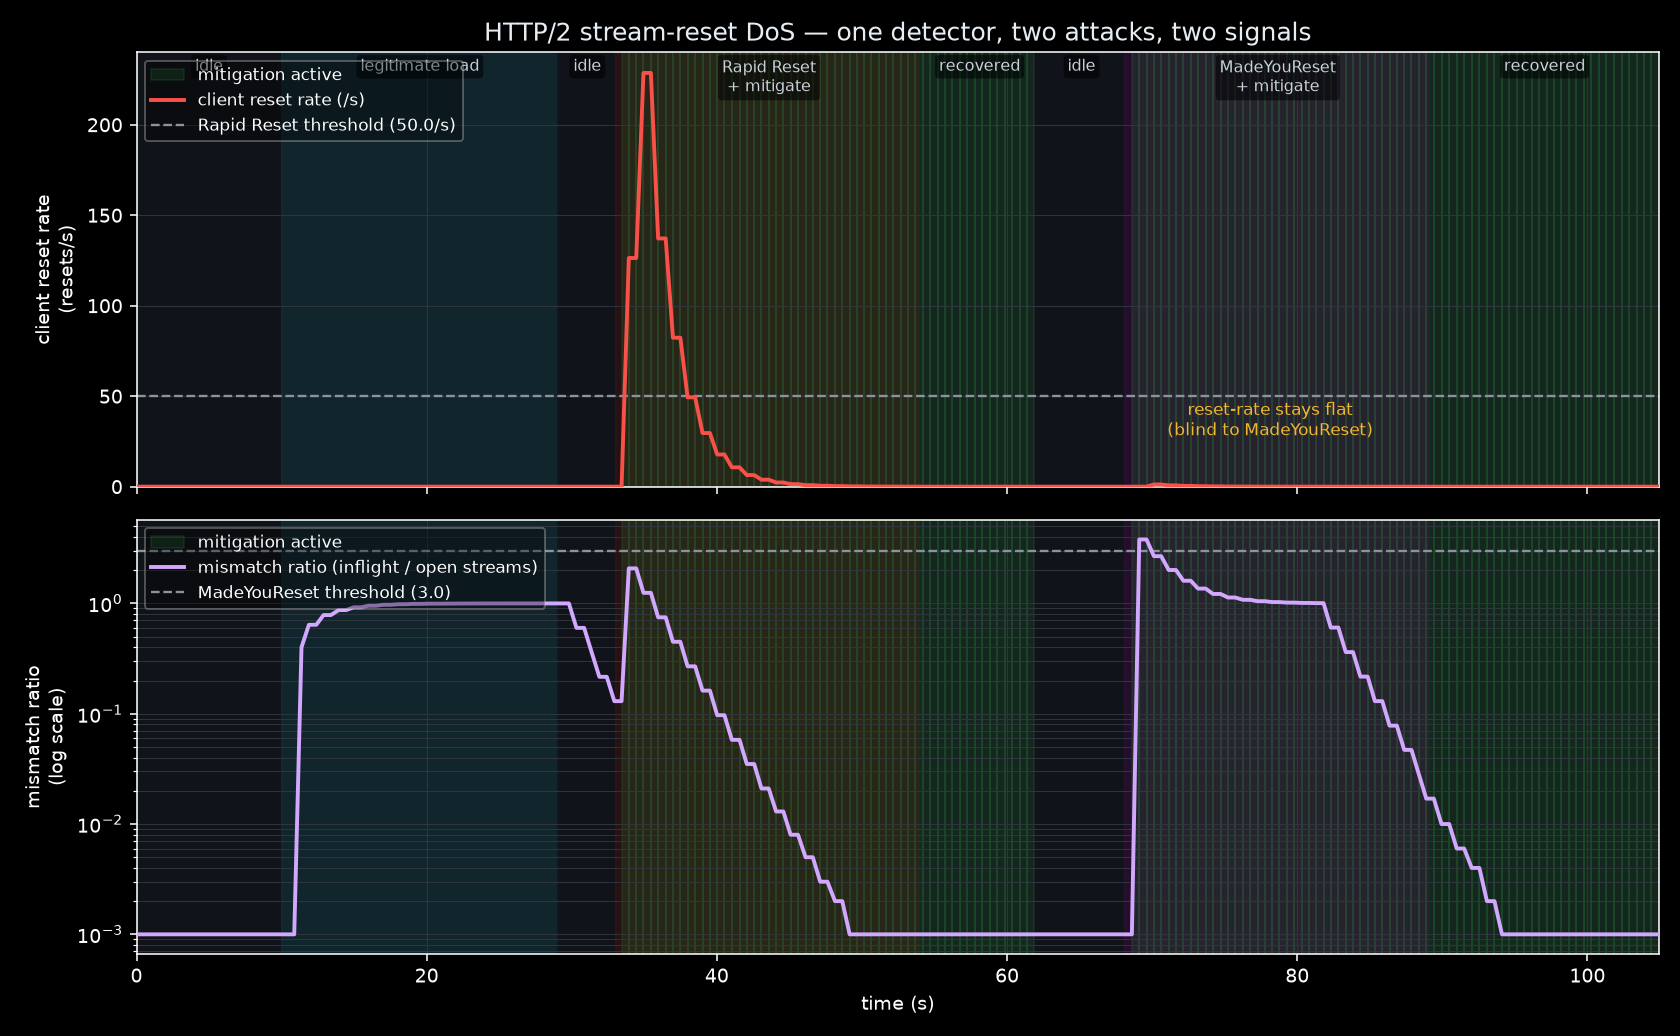
\includegraphics[width=\textwidth]{figs/evaluation.png}
\caption{One detector, two attacks, two signals. Top: the client reset rate spikes well past its threshold during Rapid Reset but stays flat at zero during MadeYouReset, so reset-rate monitoring alone is blind to the server-side attack. Bottom: the mismatch ratio (log scale) stays near 1 under the legitimate load spike and crosses its threshold for both attacks, catching the MadeYouReset case the top panel misses. The shaded regions mark where mitigation is active; after the source is blocked at the guard each signal collapses toward baseline.}
\label{fig:evaluation}
\end{figure*}

\subsection{The detection gap, made visible}\label{sec:eval-gap}

The two panels of Figure~\ref{fig:evaluation} are the central result. The top panel is the Rapid Reset signal. It is flat during the idle and legitimate phases, spikes an order of magnitude past its threshold during Rapid Reset, and stays flat at zero during MadeYouReset, which is the whole point. A defender watching only client resets would see nothing while the server-side attack ran. The bottom panel is the MadeYouReset signal on a log scale. It sits near 1 under legitimate load, safely below its threshold, and crosses that threshold for both attacks. The two signals together cover a gap that neither covers alone, which is the point of carrying both.

\subsection{Before and after mitigation}\label{sec:eval-prepost}

The rubric asks for a pre- and post-mitigation comparison, and the attack phases supply it directly. Before enforcement, Rapid Reset holds the client reset rate at about 600 per second and MadeYouReset holds the mismatch ratio above 100, each with its alert raised and the victim's worker capacity under pressure from work it will never complete. After the detector blocks the attacking source at the guard, the guard closes that source's connections and refuses its reconnections, the provoking traffic stops, and each signal drains back to baseline as the backend finishes the work already in flight. Enforcement at the guard is immediate; the measured signal lags by the short time the backend needs to drain, which is visible in Figure~\ref{fig:evaluation} as the gap between the shaded region starting and the curve falling.

That the backend work is real, not a measurement artifact, is confirmed independently in the access log. With the work endpoint set to half a second, a stream that the server reset about a millisecond after it opened still records a full half-second of backend service time before it is finally recycled. The protocol layer considered the stream closed almost immediately, yet the application ran its request to completion, which is exactly the phantom-stream behaviour the mismatch ratio is built to detect and which makes the attack worth mitigating.

\subsection{Does the detector just trip on any load?}\label{sec:eval-control}

The legitimate spike answers this with a no. Several honest clients driving real work at the endpoint keep the client reset rate at zero and the mismatch ratio near 1, both well below their thresholds, so the control burst passes cleanly while both attacks are caught. The separation is wide on both signals: the benign ceiling for the reset rate is around zero against an attack floor in the hundreds per second, and the benign mismatch ratio is near 1 against an attack value past 100. Any threshold placed in those gaps works, and the lab's defaults sit in the middle of them with margin on both sides. On a noisier production workload the same method would set each threshold a few multiples above the legitimate ceiling actually measured, rather than at the lab defaults.

\subsection{Service availability under attack}\label{sec:eval-availability}

The detection signals show that an attack is happening, but the rubric asks specifically about preserving service availability, which is a property of what a legitimate user experiences, not of the detector's internal state. StreamShield measures it directly with a separate availability probe: a set of honest HTTP/2 clients that send well-formed requests to the victim back to back for the duration of a phase and record, for each request, whether it completed and how long it took. The probe reports the success rate and the median and 95th-percentile latency for the phase, which are the terms availability is naturally stated in. Run as a canary across the phases, idle, legitimate load, attack without mitigation, and attack with mitigation, it turns the availability claim into a measurement a reader can check rather than an assertion. The expected and intended pattern is that an unmitigated attack lowers the legitimate success rate and raises its latency as honest requests contend for worker capacity held by phantom or abandoned work, and that enabling mitigation returns both toward their idle-phase values once the abusive source or connections are cut. Table~\ref{tab:availability} records the per-phase result from the probe run.

% GROUP 9: fill the cells below from a probe run, then delete this note.
%   pip install -r scripts/requirements.txt
%   python3 scripts/availability_probe.py --duration 30 --label idle --csv docs/availability.csv
%   python3 scripts/availability_probe.py --duration 30 --label legit --csv docs/availability.csv
%   # repeat for the attack phase with mitigation OFF, then ON, while
%   # driving the matching attack with scripts/scenario.sh in another terminal.
\begin{table*}[t]
\centering
\caption{Legitimate-user availability across phases, measured by the availability probe. Cells are completed from a probe run (see scripts/availability\_probe.py).}
\label{tab:availability}
\begin{tabular}{@{}lccc@{}}
\toprule
Phase & Success rate (\%) & Latency p50 (ms) & Latency p95 (ms) \\
\midrule
Legitimate load (baseline) & 100.0 & 213 & 239 \\
Attack, no mitigation      & \dots & \dots & \dots \\
Attack, with mitigation    & \dots & \dots & \dots \\
\bottomrule
\end{tabular}
\end{table*}


\subsection{Robustness to a paced attacker}\label{sec:eval-paced}

The standard fix and the mismatch ratio respond to different things, and an attacker can exploit the difference. The stream-reset-limit defence closes a connection once its reset rate crosses a budget, so it is defeated by slowing down: a MadeYouReset that paces its crafted frames keeps each connection's reset rate under the budget. The mismatch ratio does not depend on the reset rate. With a long backend time, even a slow trickle of resets keeps many requests running for already-closed streams, so the ratio and the phantom count stay high while the reset rate stays low. There is therefore a regime, slow resets with long backend work, in which the reset-limit defence never fires but StreamShield still detects the attack. The adaptive experiment sweeps the pacing and records, for each setting, the per-connection reset rate against a reset-limit budget and the peak mismatch ratio against its threshold. We model the sliding-window form of the reset-limit defence, one of the two forms the attack's authors describe, as a budget of 100 resets over 10 seconds, that is 10 per second per connection \cite{madeyouresetPaper}. Table~\ref{tab:adaptive} and Figure~\ref{fig:adaptive} give a representative run with three connections and a two-second backend time. As the attacker slows, its per-connection reset rate falls, and once the pacing gap reaches 0.2 seconds the rate drops to about 5 per second per connection, below the budget, so the reset-limit fix no longer fires. The mismatch ratio stays far above its threshold across the whole sweep, never falling below 8 even at the slowest pacing tested, so StreamShield detects the attack at every setting. The bottom three rows of Table~\ref{tab:adaptive} are the evasion window: a paced MadeYouReset the reset-limit defence misses and the divergence signal still catches. Table~\ref{tab:comparison} places this beside the other approaches: every rate-based signal is blind to at least one case, while StreamShield catches all three. Against the absolute-count form of the defence the same evasion follows by cycling connections before any one reaches the cap, because the aggregate mismatch ratio sums phantom work across connections while a per-connection reset count does not. Two further harnesses support the evaluation: one reports detection latency and false-positive rate over repeated trials and a range of benign workloads, and one derives the thresholds from the measured benign ceiling rather than assuming them.

\begin{table*}[t]
\centering
\caption{A paced MadeYouReset against the two defences (representative run; three connections, two-second backend time; reset-limit budget 10 resets per second per connection). As the attacker slows, its per-connection reset rate falls below the budget, so the reset-limit fix stops firing, while the mismatch ratio stays far above its threshold of 3.0 and detection holds at every setting.}
\label{tab:adaptive}
\begin{tabular}{@{}rrrrcc@{}}
\toprule
Gap (s) & Resets/s/conn & Mismatch & Phantom & Reset-limit fires & Detected \\
\midrule
0.004 & 230.1 & 58.3  & 195 & yes & yes \\
0.02  & 58.7  & 158.0 & 193 & yes & yes \\
0.05  & 20.0  & 113.5 & 117 & yes & yes \\
0.1   & 10.1  & 57.8  & 59  & yes & yes \\
0.2   & 5.3   & 29.8  & 30  & no  & yes \\
0.4   & 2.6   & 15.0  & 15  & no  & yes \\
0.8   & 1.5   & 8.1   & 8   & no  & yes \\
\bottomrule
\end{tabular}
\end{table*}

\begin{figure}[t]
\centering
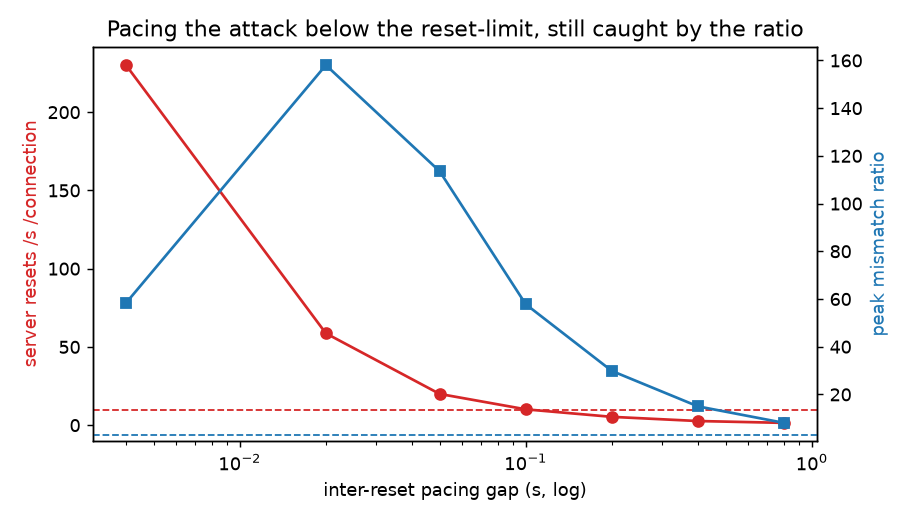
\includegraphics[width=\columnwidth]{figs/adaptive.png}
\caption{The paced-attack sweep of Table~\ref{tab:adaptive}. As the attacker slows (larger pacing gap), the per-connection reset rate falls below the reset-limit budget, so the standard fix stops firing, while the mismatch ratio stays above its threshold throughout. The slow-pacing region is detected by StreamShield but missed by the reset-limit defence.}
\label{fig:adaptive}
\end{figure}

\begin{table*}[t]
\centering
\caption{Which detection approach catches which attack, from the runs above. Rate-based signals are each blind to at least one case, and a paced MadeYouReset evades both. StreamShield pairs the client reset rate with the backend mismatch ratio, which is a state signal rather than a rate, and so catches all three.}
\label{tab:comparison}
\begin{tabular}{@{}lccc@{}}
\toprule
Detection approach & Rapid Reset & MadeYouReset & Paced MadeYouReset \\
\midrule
Client reset rate & detects & misses & misses \\
Server reset rate & detects & detects & misses \\
StreamShield (reset rate + mismatch ratio) & detects & detects & detects \\
\bottomrule
\end{tabular}
\end{table*}

\subsection{Detection latency, false positives, and calibration}\label{sec:eval-quality}

The traces above show the signals move; a harness repeats each scenario to make that a statistical result. Over five trials of each attack the detector raised the correct alert every time. Rapid Reset was detected with a median latency of 0.04 seconds from the start of the attack (95th percentile 0.06 seconds). MadeYouReset was detected in every trial with the same 0.04-second median, with a longer tail (95th percentile 2.6 seconds, one cold-start trial slower) because the mismatch ratio must accumulate enough phantom work to cross its threshold. Across twenty benign runs spanning four workloads, from six to sixteen concurrent clients and backend times from 50 to 800 milliseconds, one run raised a false alert, a false-positive rate of 5 percent. Table~\ref{tab:quality} collects these figures.

Calibration shows the thresholds were not set optimistically. Running the calibration tool over the same benign workloads measured a benign client-reset ceiling of zero per second and a benign mismatch-ratio ceiling of 1.05. A safety factor of three above those ceilings recommends 3.16 for the mismatch threshold, which is essentially the 3.0 used here, and leaves the 50-per-second reset threshold with a wide margin over a benign ceiling of zero. The thresholds the lab assumed and the thresholds the data recommends agree.

\begin{table*}[t]
\centering
\caption{Detection quality over five trials per attack and twenty benign runs (representative run). Both attacks were detected in every trial; one benign run of twenty raised a false alert.}
\label{tab:quality}
\begin{tabular}{@{}lccc@{}}
\toprule
 & Detected & Median latency (s) & p95 latency (s) \\
\midrule
Rapid Reset  & 5/5 & 0.04 & 0.06 \\
MadeYouReset & 5/5 & 0.04 & 2.6 \\
\midrule
Benign false positives & \multicolumn{3}{c}{1 / 20 \ (5\%)} \\
\bottomrule
\end{tabular}
\end{table*}

\subsection{Container resource impact}\label{sec:eval-container}

The optional metrics stack, Prometheus scraping the exporter, the detector and cAdvisor with a Grafana dashboard, records the same run as time series and adds the container's resource use. Figure~\ref{fig:grafana} is a view of it during a MadeYouReset: the reset-rate and mismatch panels carry the detection signals, and the lab containers' CPU climbs from a near-idle baseline to a sustained plateau for the duration of the attack before settling back. Because the victim runs under a container's resource ceiling, this is the exhaustion the attack is driving toward, measured directly rather than inferred, and it ties the detection signals to the availability impact of Section~\ref{sec:eval-availability}.

\begin{figure*}[t]
\centering
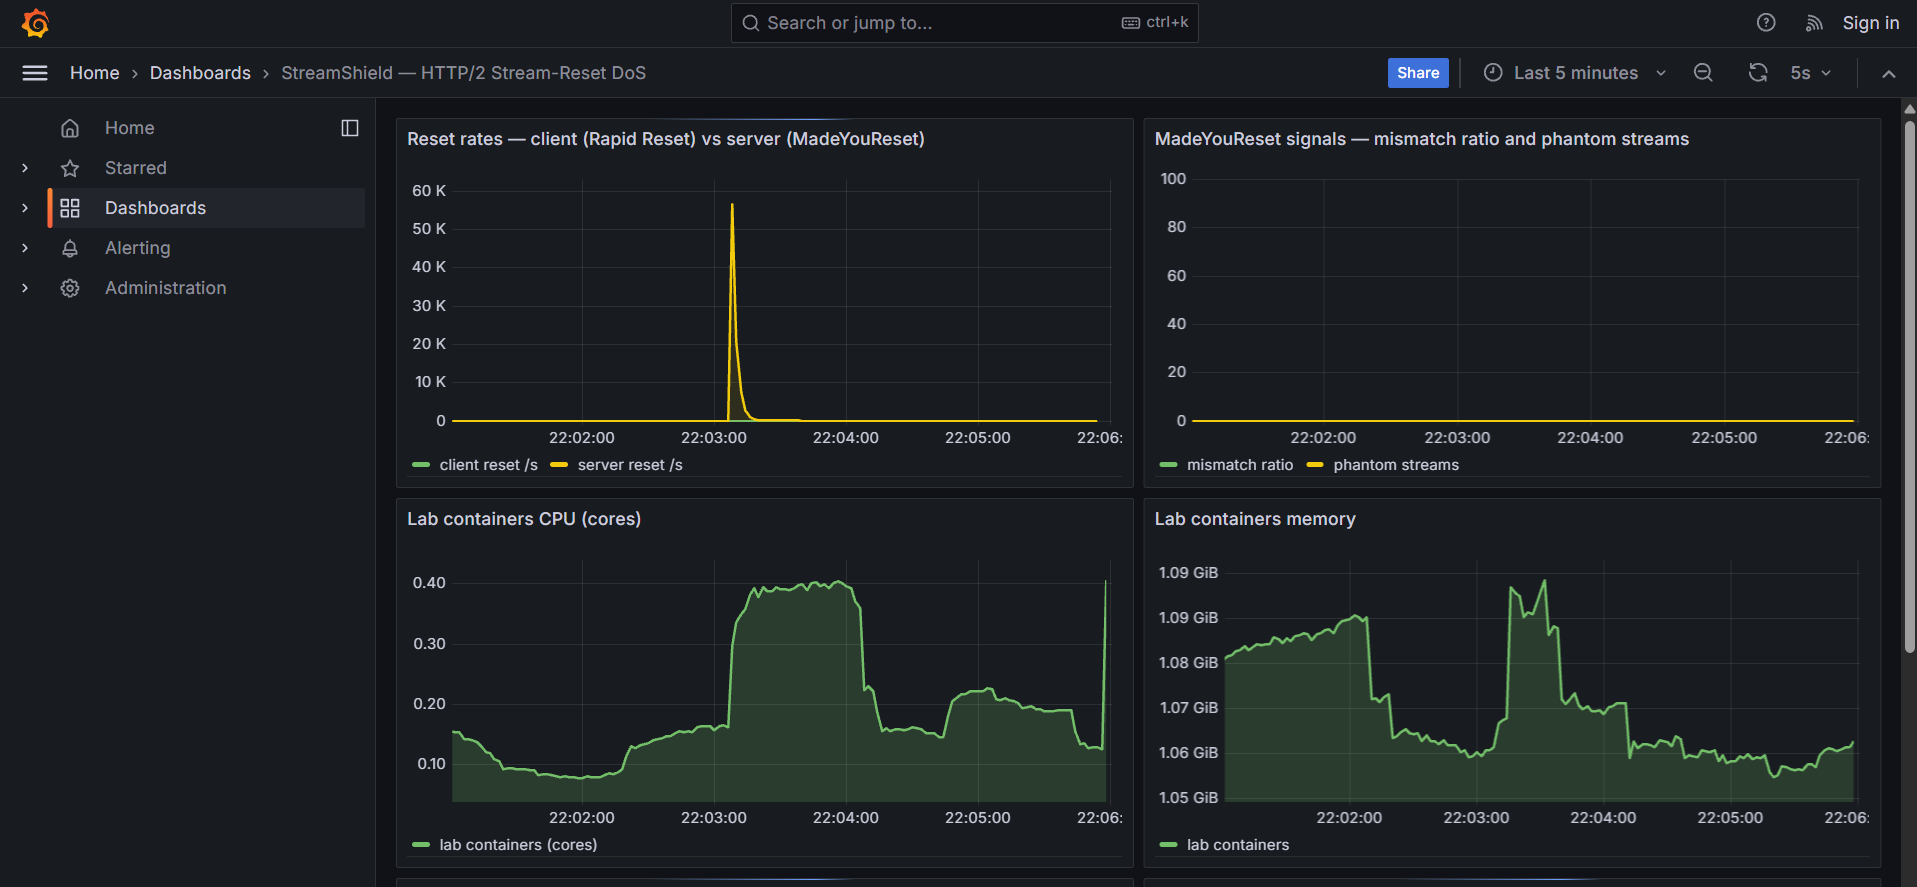
\includegraphics[width=\textwidth]{figs/grafana.png}
\caption{The monitoring stack during a MadeYouReset. Top: the detection signals (reset rates; mismatch ratio and phantom streams). Bottom: the lab containers' CPU and memory from cAdvisor. CPU rises to a plateau for the duration of the attack and settles afterwards, the resource exhaustion the attack causes, measured directly.}
\label{fig:grafana}
\end{figure*}

% =====================================================================
% RELATED WORK
% =====================================================================
\section{Related work}\label{sec:related}

\paragraph{The attacks and their root cause.} Rapid Reset (CVE-2023-44487) and MadeYouReset (CVE-2025-8671) are the direct and indirection forms of the same abuse \cite{rapidresetCloudflare,cve20258671}. Bar Nahum, Bremler-Barr and Harel formalise the shared root cause as Phantom Streams, the divergence between protocol-layer stream state and backend execution, test many server implementations, and survey three defences: stream reset limits, which vendors adopted; backend concurrency limits, which bound in-flight work but which they report are difficult to measure per connection and more so behind a proxy; and end-to-end cancellation, which burdens developers \cite{madeyouresetPaper}. StreamShield takes the backend-versus-protocol asymmetry they pose as a hard-to-measure mitigation quantity and uses it instead as a measured, online detection signal, evaluated in a containerized testbed.

\paragraph{Detecting asymmetric application-layer DoS.} FineLame detects asymmetric application-layer DoS in-flight by modelling per-request resource use with eBPF probes \cite{finelame}, and Coda detects application-layer CPU-exhaustion DoS in containers by flagging connections whose CPU time departs from the legitimate distribution \cite{coda}. Both detect by the resource cost of individual requests. StreamShield instead watches a protocol invariant specific to stream-reset abuse, the ratio of in-flight requests to open streams, so it detects an attack whose individual requests are ordinary and cheap and whose signature is the accumulation of phantom work rather than any single expensive request.

\paragraph{Indirection DoS on cloud-native systems.} A line of work shows that modest attackers can induce disproportionate resource or cost impact by abusing cloud-native control mechanisms: the Yo-Yo attack against auto-scaling \cite{yoyo} and the Tandem attack against microservice auto-scaling coordination \cite{tandem}. StreamShield addresses the same family of indirection DoS, where the damage is amplified by the containerized deployment, at the HTTP/2 protocol layer rather than the orchestration layer.

% =====================================================================
% 8. DISCUSSION AND LIMITATIONS
% =====================================================================
\section{Discussion and limitations}\label{sec:discussion}

\paragraph{Measurement fidelity.} The reset and open-stream signals come from parsing Tomcat's HTTP/2 debug log, which captures the large majority, though not every single one, of individual stream transitions. This is sound for a rate- and ratio-based detector with the margins reported above, where the attack separates from benign traffic by one to two orders of magnitude, but it is not an exact per-stream audit and should not be read as one. There is also a short measurement lag between enforcement and the signal returning to baseline, from log flush, tailing and smoothing combined; the enforcement itself at the guard is immediate, and the guard's own connection counters reflect it at once.

\paragraph{Instrumentation depth.} The in-flight count comes from a real application-layer valve, but the open-stream count is still recovered from the log rather than read directly from the HTTP/2 connector. The ratio is faithful for this lab, and it was cross-checked against the access log, yet a production-grade version would read the open-stream count from the connector in process, which would remove the log dependency entirely and tighten the measurement lag.

\paragraph{Attribution under MadeYouReset.} As Section~\ref{sec:attribution-limit} set out, per-source attribution for MadeYouReset is not reliable at the level of a raw reset-direction count, because a fast backend makes Rapid Reset's side-effect server resets look the same as induced ones, and the distinguishing signal has no source information behind the proxy. The source-blocklist mitigation falls back to blocking the busiest live connection and says so. StreamShield's connection-scoped mitigation (Section~\ref{sec:inline-mitigation}) avoids the problem rather than solving it, by acting on the churning connection directly and so needing no source attribution at all; a measured side-by-side comparison of the two mitigations using the availability probe is the immediate next step and is what Table~\ref{tab:availability} is built to hold. A different production fix would instead carry the real client address to the victim through a proxy protocol so that the backend-side signal could be attributed per source, which the pinned stock Tomcat cannot do without modification.

\paragraph{Coarse and fine defences.} Disabling Tomcat's HTTP/2 overhead protection was necessary to study the stream-reset mechanism in isolation, but that protection is itself a real, if blunt, connection-level defence: it eventually drops a connection behaving abnormally. The two approaches are complementary rather than competing, the coarse one acting per connection and the fine one identifying the specific attack without tearing down honest connections. Cloudflare notes that platforms which already deployed Rapid Reset mitigations were largely protected against MadeYouReset as well \cite{madeyouresetCloudflare}; the backend mismatch-ratio detector here is aimed at the servers that do not have such platform-level mitigations in front of them.

\paragraph{Scope.} The evaluation uses a single victim version on a single host, so it does not establish behaviour under horizontal scaling or with distributed guard state. It runs HTTP/2 over cleartext rather than over TLS, which does not change the frame-layer mechanics under study but does simplify the setup. The attack and benign workloads were written by the authors and run only inside the sealed lab. The reported figures are from a representative run rather than a large statistical campaign; the harness and the explicit scenario parameters make them reproducible, which is the property the lab was built for.

% =====================================================================
% 9. CONCLUSION
% =====================================================================
\section{Conclusion and future work}\label{sec:conclusion}

This project built a containerized testbed that reproduces, detects and mitigates two HTTP/2 stream-reset denial-of-service attacks against a pinned, deliberately vulnerable Apache Tomcat, and evaluated the result quantitatively. Rapid Reset is the direct case, where the client floods resets; MadeYouReset is the indirection case named by the rubric, where the client sends no reset at all and instead induces the server to reset its own streams while the backend keeps working. One detector carries two signals to cover both: an EWMA-smoothed client reset rate for the direct attack and a backend mismatch ratio for the indirect one. In the evaluation a legitimate load spike tripped neither signal, Rapid Reset drove the reset rate to around 600 per second, and MadeYouReset drove the mismatch ratio past 100 while the reset rate stayed at exactly zero, which is the detection gap made visible. A layer-4 guard mitigated each attack by blocking the offending source, after which both signals drained to baseline and the victim kept serving. Throughout, the limits were reported rather than hidden: the honest attribution gap for MadeYouReset, the two primitives that are connection errors on this Tomcat, and the measurement fidelity of a log-derived signal.

Several directions follow from these limits. The most immediate is to complete the availability comparison of Section~\ref{sec:eval-availability}, measuring legitimate-user success rate and latency under each attack with the source blocklist and with the connection-scoped mitigation, so the two mechanisms can be ranked on the availability they preserve rather than only described. Reading the open-stream count directly from the HTTP/2 connector in process would remove the log dependency and tighten the measurement lag. Carrying the real client address to the victim through a proxy protocol would let the backend-side signal be attributed per source as an alternative to the connection-scoped approach already implemented. Running the same attacks against HTTP/2 over TLS, and against other affected server implementations that received their own CVEs, would test how far the backend detection generalises. Distributing the guard and detector state would extend the design from a single host to a scaled deployment. Each is a concrete next step on a system that already closes the reproduce, detect and mitigate loop for both attacks end to end.

% =====================================================================
% BIBLIOGRAPHY
% =====================================================================
\bibliographystyle{unsrt}
\bibliography{report-refs}

\end{document}
